\newpage{}

\section{Simulation Analysis}
\label{sec:simulation}
\paragraph{}


\par A software called NGSpice was exploited to simulate the AC DC converter. It is important to note that some changes were made to the circuit, from the get-go, for simplification purposes. 
\par The following table shows the results computed by the simulation: the input voltage of the secondary circuit (v(2)), the ouput voltages of the Envelope Dectector and the Voltage Regulator (v(4) and v(5), respectively).


\begin{table}[H]
  \centering
  \begin{tabular}{|c|c|}
    \hline    
    \input{../sim/sim_tab.tex}
  \end{tabular}
  \caption{Ripple and Average Voltages for Envelope and Regulator}
  \label{sim1}
\end{table}

\par The value computed for Merit was $4.03\times 10^{-2}$, which was lower than what was expected, meaning the circuit could have been more optimized. However, it was felt that the value was satisfying for the purpose of this assignment.

\begin{table}[H]
  \centering
  \begin{tabular}{|c|c|}
    \hline    
    \input{../sim/merit_tab.tex}
  \end{tabular}
  \caption{Merit calculated through NgSpice}
  \label{sim1}
\end{table}

\par The following plot shows the voltage of the transformer v(2)-v(3), the voltage of Envelope Detector v(4) and Voltage Regulator v(5).

\begin{figure}[H]
    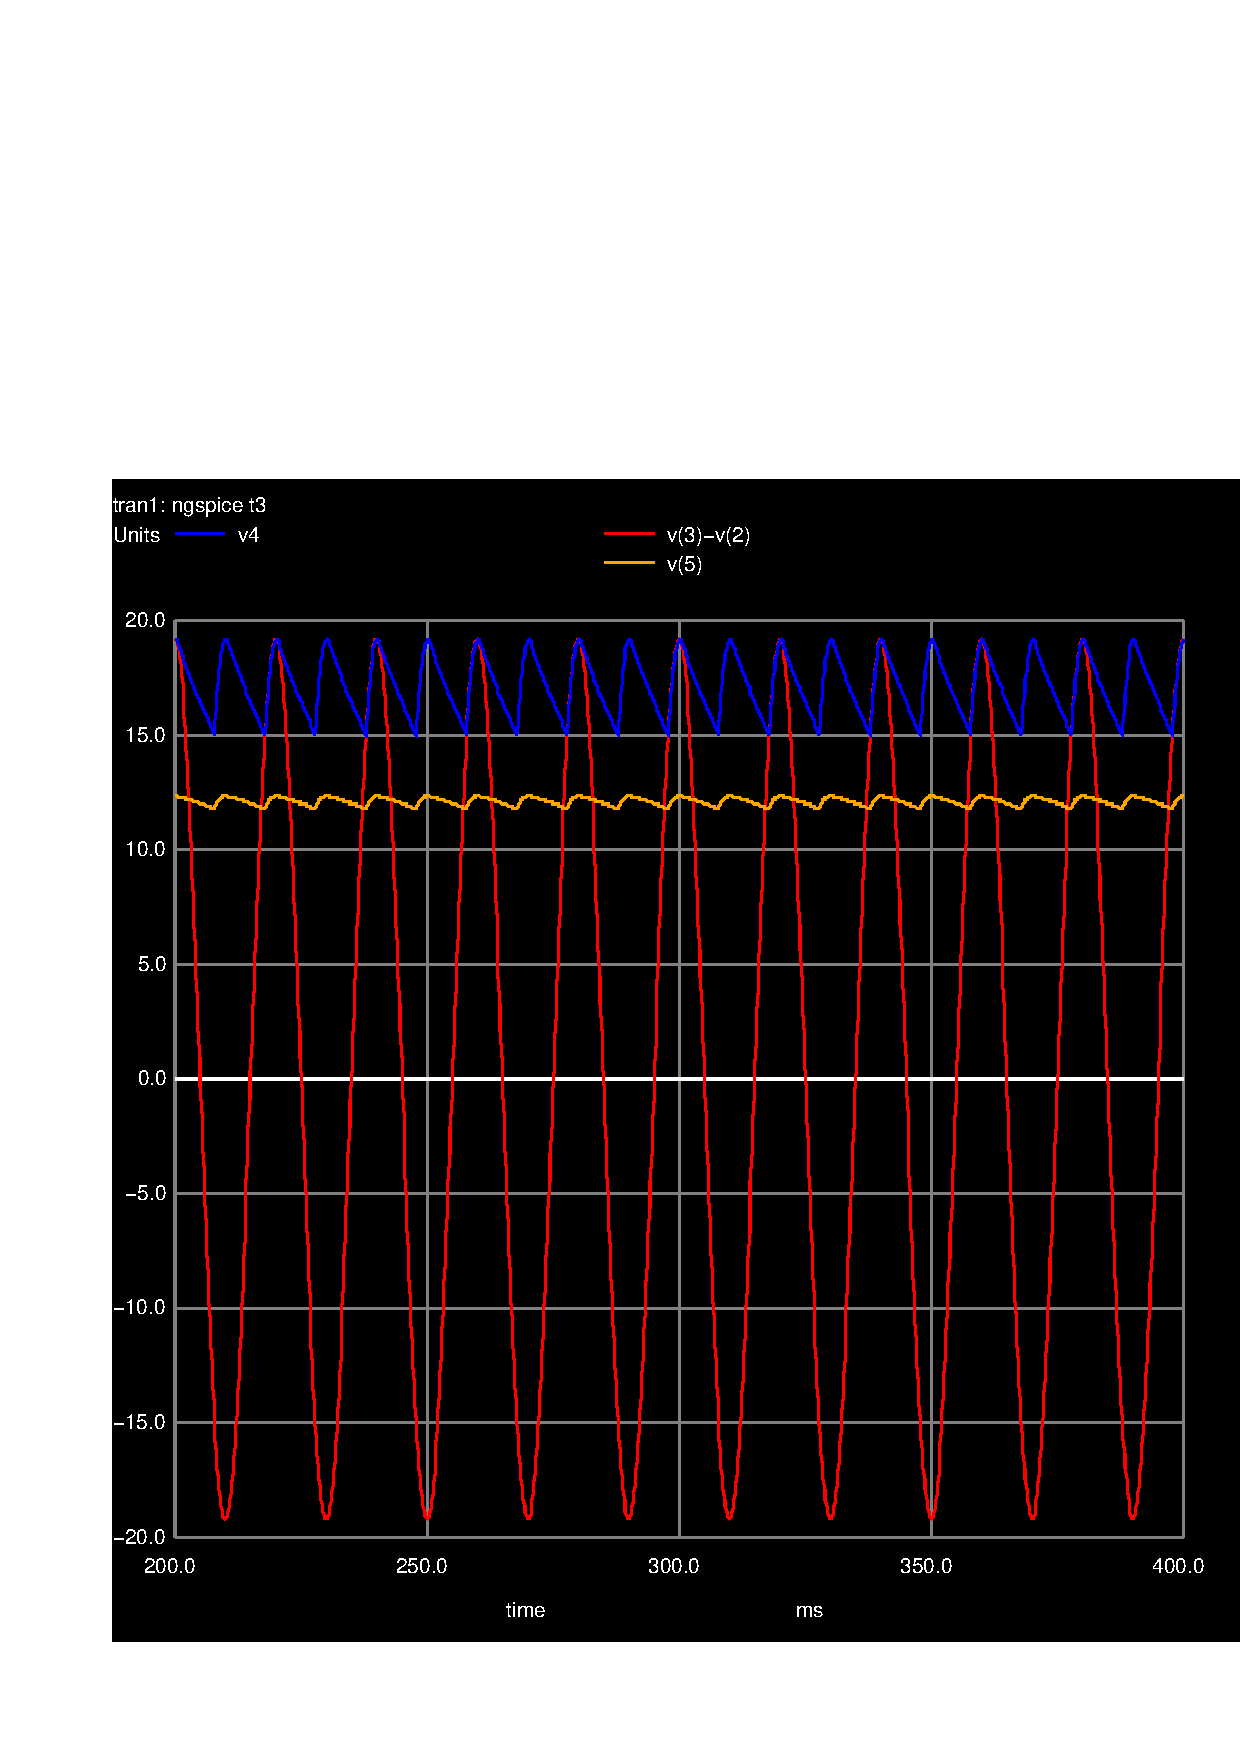
\includegraphics[width=0.495\linewidth]{../sim/comp.pdf}
    \centering
    \caption{Voltage of the rectifier, Voltage of Envelope Detector and Voltage Regulator}
    \label{mag}
\end{figure}
\par Then, the Deviation from the desired DC voltages was also plotted. The variable v(5) corresponds to $v_o$
\begin{figure}[H]
    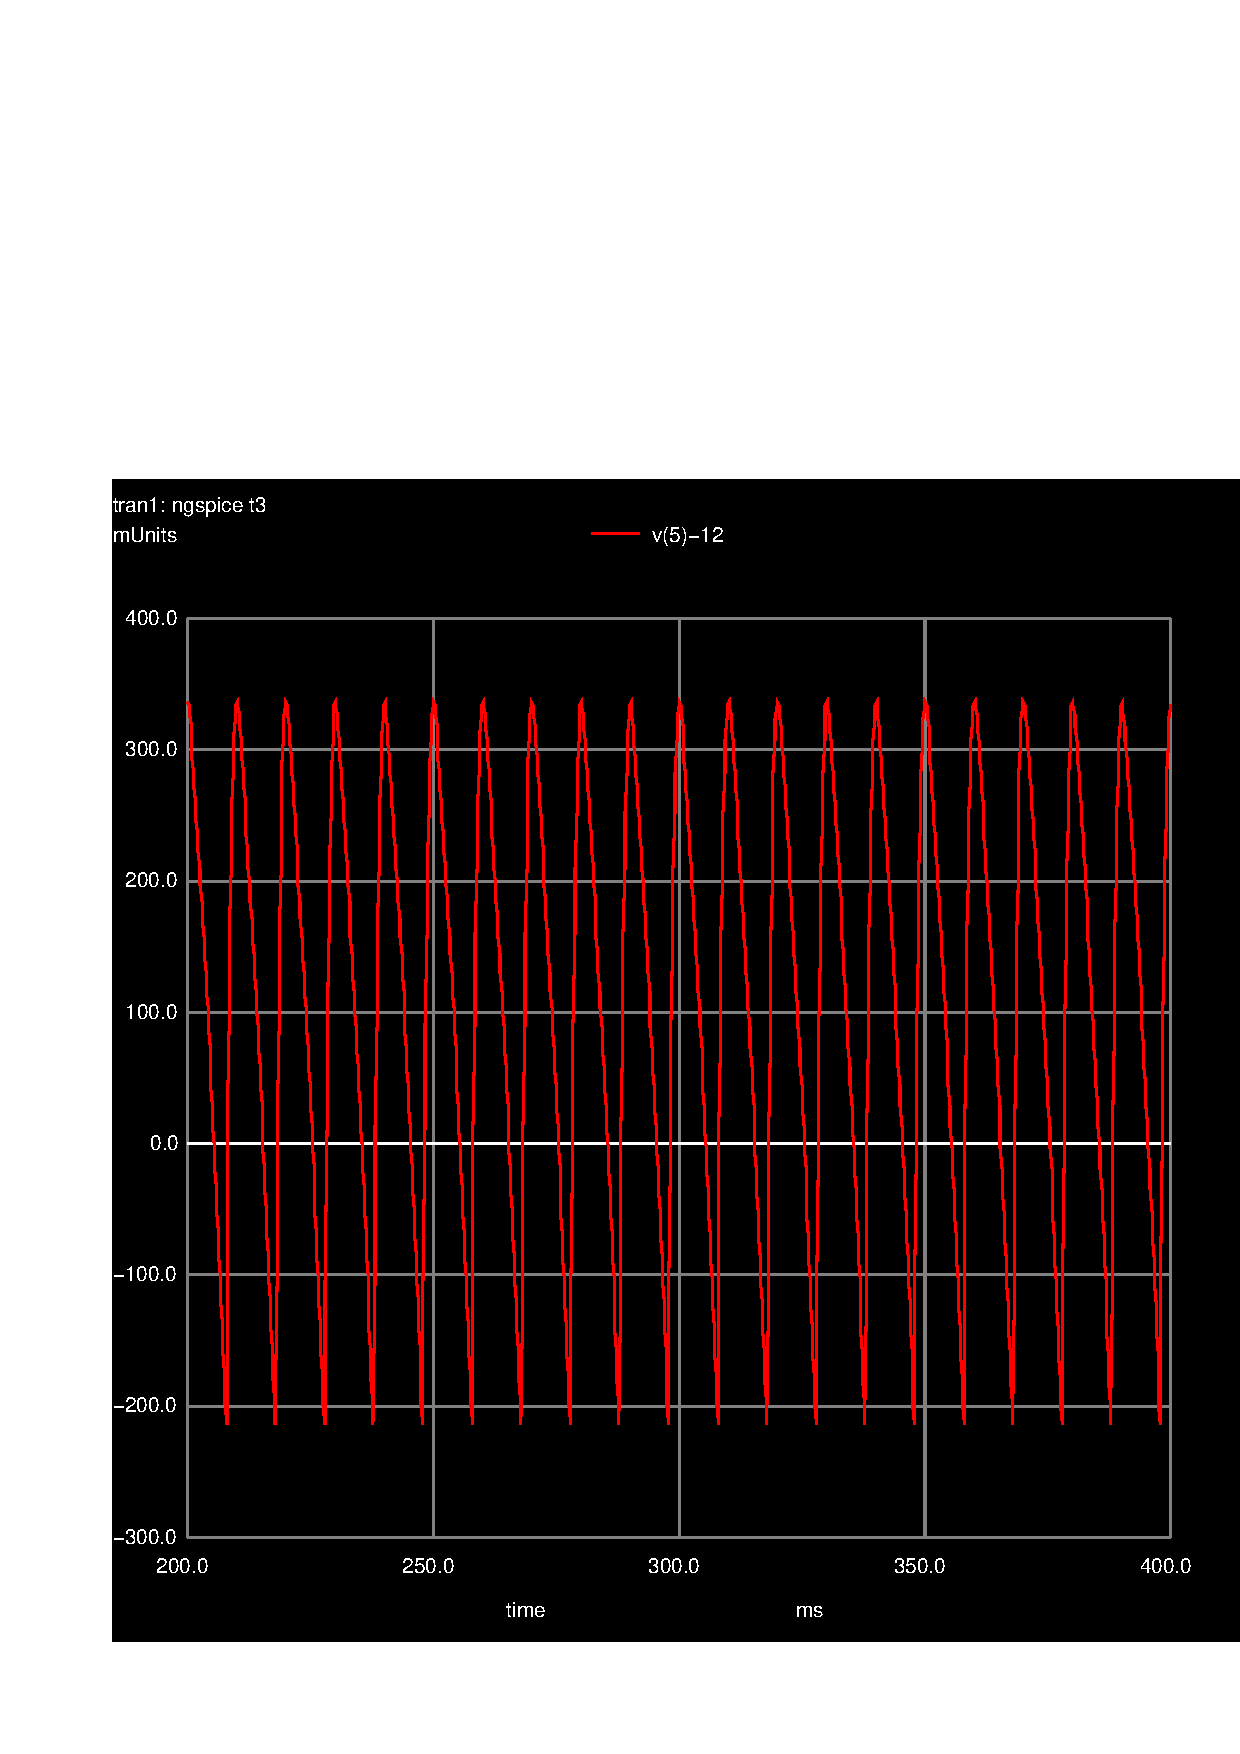
\includegraphics[width=0.495\linewidth]{../sim/dev.pdf}
    \centering
    \caption{$v_0-12$ (Deviation from the desired DC voltages)}
    \label{mag}
\end{figure}

\newpage{}

